% LTeX: language=en-GB
% !TeX root = ..\Thesis.tex
\section{Design}\label{sec:04}
The design of SteelBrew will take an Agile approach to get going with some framework for writing and running simple tests on devices written in SystemVerilog, using Java.
\subsection{Usecases}
Using SteelBrew should be as simple as possible. \cref{fig:usecases} shows an overview of the usecases for a developer.
\begin{figure}
    \centering
    \caption{Usecase diagram for SteelBrew}\label{fig:usecases}
    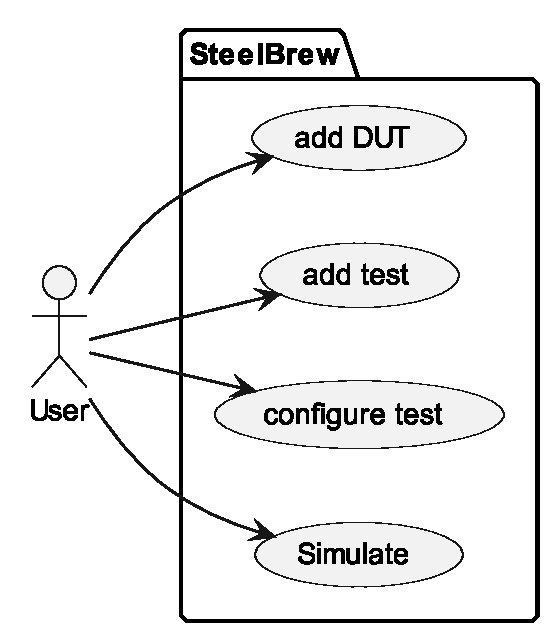
\includegraphics[width=.3\textwidth]{out/plantuml/usecase/usecase.eps}
\end{figure}
This is a simplification. As mentioned the framework is executed in Java, so to get started the user would start by creating a java project and importing SteelBrew. Hereafter the DUT is added and tests are defined and configured. A command should then execute the test and start the simulation.
\subsubsection{Adding the device under test}
\subsubsection{Adding tests}
\subsubsection{Configure tests}
\subsubsection{Simulate}